%! Author = taj
%! Date = 7/22/25

% Preamble
\documentclass[11pt]{article}

% Packages
\usepackage{amsmath}
\usepackage{graphicx}
\usepackage{float}

\title{7. Enakomerno pospešeno gibanje}
\author{Taj Šobot}

% Document
\begin{document}
    \maketitle
    \flushleft

    \section{Meritve}
    Graf x(t) za 4 različne meritve:
    \begin{figure}[H]
        \centering
        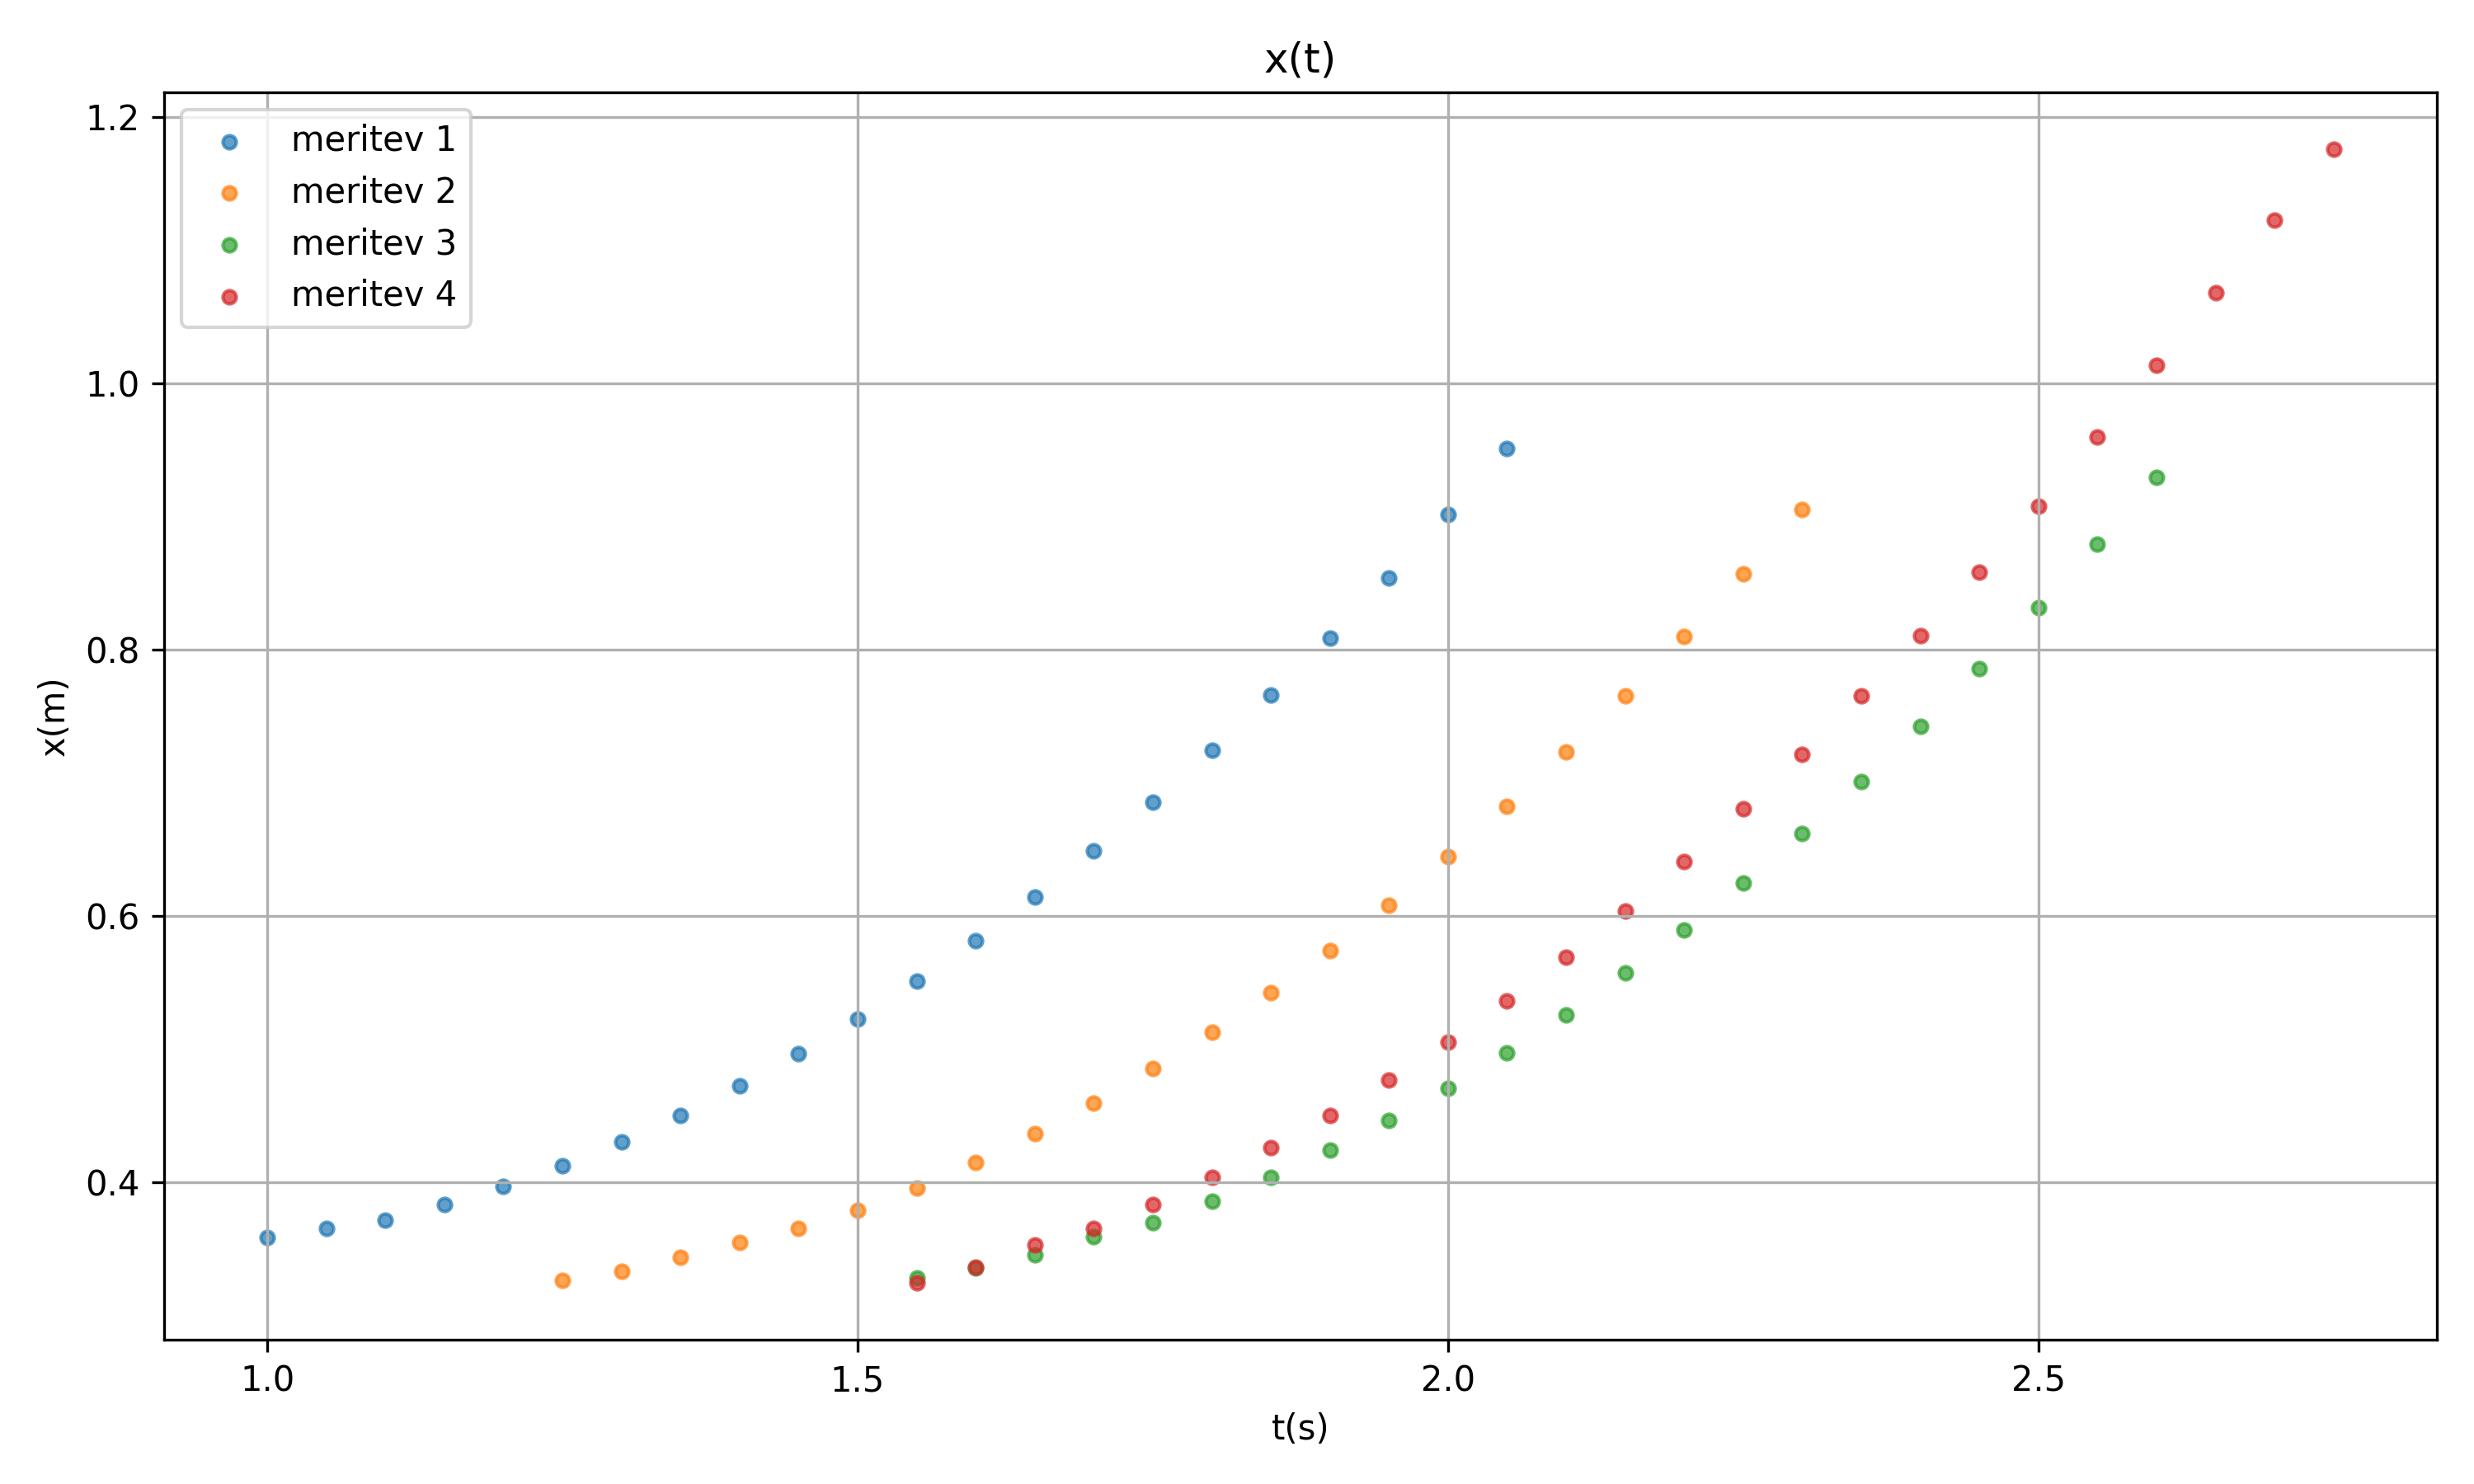
\includegraphics[width=0.9\textwidth]{xt}
        \caption{Graf x(t)}
        \label{fig:2}
    \end{figure}


\end{document}